\documentclass{easychair}
%\usepackage{rotating}
%\usepackage{pdflscape}
%usepackage{algorithm2e}
\newcommand{\easychair}{\sf{easychair}}
\newcommand{\miktex}{MiK{\TeX}}
\newcommand{\texniccenter}{{\TeX}nicCenter}
\newcommand{\makefile}{\texttt{Makefile}}
\usepackage[portuguese]{babel}
\usepackage{epsfig}
\usepackage{subfig,syntonly,amsmath,amssymb,cite,graphicx}
\usepackage{nomencl}
\usepackage[strings]{underscore}
\usepackage{float}
\usepackage{amsthm}
\usepackage{amsmath}

%\usepackage[utf8]{inputenc}  % adaptar 'a codificacao do sistema
%\usepackage[portuges]{babel}

%% Document
%%
\begin{document}
\raggedbottom

\title{Segmentação de Clientes e Previsão do Risco de Abandono Através de Análise RFM}

\titlerunning{}

% Authors are joined by \and and their affiliations are on the
% subsequent lines separated by \\ just like the article class
% allows.
%

\author{Rui Ruivo\\
Universidade de Évora\\
\url{m60739@alunos.uevora.pt}\\
}

\authorrunning{R. Ruivo}

\maketitle

%----------------------------------------------------------------------------------------------------------
\begin{abstract}
Hoje em dia, e com o aumento do negócio online, as empresas enfrentam um ambiente de mercado altamente competitivo e dinâmico, onde compreender o comportamento dos clientes tornou-se essencial para garantir vantagem competitiva. A necessidade de reter clientes existentes e prever comportamentos como o risco de abandono é mais crítica do que nunca.
Neste contexto, a análise e mineração de dados emerge como uma aliada indispensável, permitindo que que as organizações tomem decisões baseadas em evidências.

Neste artigo, são descritos os passos necessários para preparar um conjunto de dados contendo informações de transações comerciais de uma plataforma de retalho online sediada no Reino Unido. A preparação e limpeza deste conjunto de dados irá permitir realizar uma análise RFM (\textbf{R}ecência, \textbf{F}requência e Valor \textbf{M}onetário) para identificar os principais clientes e calcular o risco de cada um deles abandonar o negócio (em inglês: \textbf{\textit{customer churn}}).

Os passos descritos neste artigo são aplicáveis a qualquer tipo de negócio, sendo uma ferramenta valiosa para qualquer empresa que deseja monitorizar as tendências dos seus clientes e agir em conformidade, para evitar a perda de quota de mercado.
\end{abstract}
%----------------------------------------------------------------------------------------------------------

%----------------------------------------------------------------------------------------------------------
\section{Introdução}
Com o aparecimento da Internet, principalmente aquando da sua massificação no íncio dos anos 2000, houve uma mudança de paradigma na forma como as pessoas realizavam compras. Se até aí a realização de compras implicava a deslocação a uma loja ou a uma grande superfície comercial (o que se traduzia num aumento de custos, como despesas com combustível e a perda de tempo associada à deslocação), a Internet permitiu o aparecimento de plataformas de \textit{E-commerce} que ofereciam aos utilizadores a possibilidade de realização de compras dos mais variados artigos sem que tivessem de sair de casa.

De acordo com dados do \textit{Eurostat}, entre 2010 e 2023 houve um aumento de 22\% no número de utilizadores que compraram ou encomendaram bens ou serviços no último ano\cite{eurostat}. Esse crescimento, aliado a inovações tecnológicas como os \textit{smartphones}, \textit{apps} e pagamentos online seguros, influenciou os comportamentos de consumo e preferências dos utilizadores.

Neste novo mundo de rápida evolução tecnológica, torna-se necessário que as organizações adotem técnicas que lhes permitam compreender os comportamentos dos consumidores, identificando não só os seus clientes mais valiosos, mas também quais os clientes que se encontram em risco de deixar de usar os seus serviços, cancelar uma assinatura ou simplesmente parar de fazer compras. Felizmente para as organizações, a interação dos seus clientes com os seus serviços deixa uma riqueza de dados que podem ser explorados para caracterizar os seus hábitos e ajudar a definir estratégias personalizadas para aumentar não só a retenção, fidelização e o lucro, mas também a criação de novos produtos que vão ao encontro dos gostos dos clientes.

Para solucionar este problema, e após a realização de uma cuidadosa pesquisa sobre o tema nos mais variados artigos cientificos (muitos dos quais podem ser encontrados nas referências bibliográficas deste artigo), tomou-se a decisão de preparar o conjunto de dados para permitir a recolha de informação para cada cliente sobre a data da sua última compra, qual a frequência com a qual o cliente interage com a organização (ou seja, quantas vezes realizou compras) e qual o valor total que o cliente gastou no conjunto de todas as suas compras, este procedimento é a base da análise RFM. Além disso, com base na pontuação RFM obtida, é feita a segmentação dos clientes em grupos através de \textit{k-means clustering} e calculado um valor normalizado de probabilidade de abandono (o chamado \textbf{\textit{customer churn}}) para cada cliente com base nas pontuações RFM. O último passo passa pela avaliação do nosso modelo através da utilização de algoritmos classificadores, como \textit{J48}, \textit{Logistic} (implementação do Weka de regressão logística), \textit{RandomForest} e \textit{SMO}. A metodologia adotada, bem como os passos tomados para a preparação do conjunto de dados, serão apresentados mais à frente neste artigo.

Na realidade, a utilização apenas das componentes de Recência, Frequência e valor Monetário, embora sejam fáceis de calcular e perceber, apenas cobrem um aspeto do comportamento dos clientes. Na obtenção de modelos de previsão com alta qualidade, são necessários mais dados acerca das necessidades dos utilizadores, as suas opiniões, características socio-económicas e dados relacionais, entre outros\cite{SGEM2008}. Na realização deste estudo, iremos focar-nos na previsão do risco de abandono apenas com base nas métricas RFM, dado que o nosso conjunto de dados tem informação limitada sobre as transações de clientes por questões de privacidade dos dados. No entanto, os procedimentos realizados aqui podem ser estendidos a outros estudos, dependendo sempre da estratégia empresarial tomada por cada organização.

%----------------------------------------------------------------------------------------------------------

%----------------------------------------------------------------------------------------------------------
\section{Preparação dos Dados para Análise}
\subsection{Remoção das instâncias com valores em falta}

Antes de procedermos à nossa análise, é necessário realizar a limpeza do nosso conjunto de dados. O conjunto de dados é composto por 1048124 instâncias e 8 atributos, com as seguintes características:

\begin{enumerate}
    \item \textbf{Invoice}: Atributo nominal. Número de fatura que identifica cada compra realizada por determinado cliente. As devoluções são identificadas pelo número de fatura precedido por 'C'.
    \item \textbf{StockCode}: Atributo nominal. Corresponde ao código identificador de cada artigo.
    \item \textbf{Description}: String que descreve o artigo comprado.
    \item \textbf{Quantity}: Atributo numérico. Corresponde à quantidade do artigo. Caso a fatura seja um cancelamento ou devolução, o número é negativo.
    \item \textbf{InvoiceDate}: String que indica a data da fatura.
    \item \textbf{Price}: Atributo numérico. Indica o preço por unidade do artigo comprado.
    \item \textbf{Customer}: Atributo numérico que identifica unicamente cada cliente.
    \item \textbf{Country}: Atributo nominal. Indica o país de residência do cliente.
\end{enumerate}

O primeiro passo na limpeza dos dados é a identificação e remoção de instâncias com valores em falta. Ora, como o nosso objetivo final é a segmentação de clientes, devemos olhar para a coluna \textit{"Customer"} e remover todas as instâncias sem a informação relativa ao cliente. Caso se mantivesse essa informação, o agrupamento dos dados por cliente iria reunir todas as compras sem número de cliente num só registo, como se se tratasse de um cliente apenas, o que iria tornar a nossa analise menos precisa.
Para realizar a limpeza dos dados em falta, iremos utilizar o Microsoft Excel. Começamos por abrir o programa filtramos os dados vazios pela coluna \textit{"Customer ID"}. A figura \ref{fig1} mostra a aplicação do filtro:

\begin{figure}[H]
    \begin{centering}
    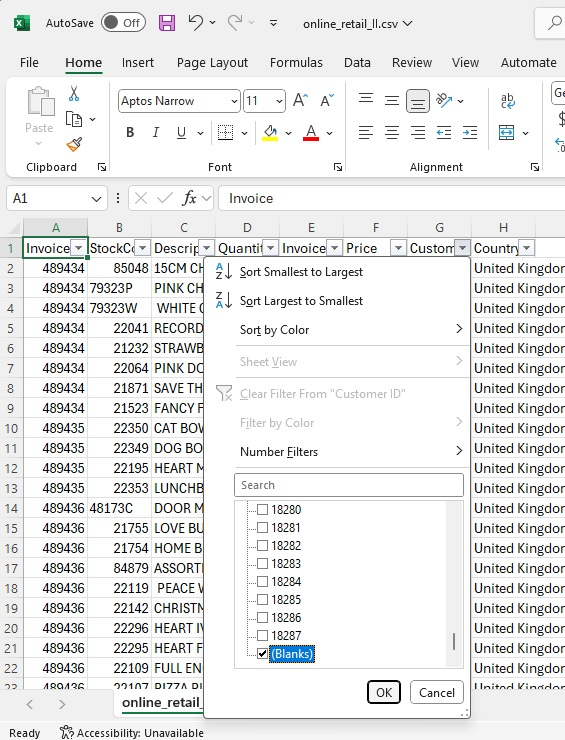
\includegraphics[width=0.55\linewidth]{imagens/figure1.jpg}\label{cap-2-fig1}
    \captionof{figure}[LOF entry]{Filtro das instâncias com \textit{"Customer ID"} vazio.}
    \label{fig1}
    \end{centering}
\end{figure}

Após filtrarmos as linhas, selecionamos todas as que queremos eliminar e clicamos em \textit{"Delete"} no teclado. O ficheiro passou das suas 1048124 instâncias para 811894 instâncias.

\subsection{Remoção das instâncias correspondentes a cancelamentos e cálculo de valores de RFM por cliente}

De seguida, devemos eliminar também as instâncias dos nossos dados que dizem respeito a devoluções e cancelamentos de encomendas.  Para tal, utilizamos um \textit{script} Python desenvolvido para esse efeito. Esse script irá também calcular os valores de Recência, Frequência e valor Monetário para cada cliente, que irão ser importantes para a análise posterior.
No fim de corrermos o \textit{script} iremos ter um ficheiro .csv com os cálculos RFM para cada cliente e sem as linhas referentes a cancelamentos.

Com a realização desta limpeza do conjunto de dados, estamos prontos a passar aos próximos passos, com o software \textit{Weka}\cite{weka}.

%----------------------------------------------------------------------------------------------------------

\subsection{Remoção de duplicados através do Weka}

Para procedermos à análise do nosso \textit{dataset}, iremos precisar de o carregar no \textit{Weka}. Para tal, depois da abertura do programa, devemos carregar no botão \textit{"Explorer"}, de seguida, clicamos no botão \textit{"Open file..."} e escolhemos qual o ficheiro abrir. Após a abertura do ficheiro, a janela do \textit{"Explorer"} deverá mostrar algo como representado na figura \ref{fig2} :

\begin{figure}[H]
    \begin{centering}
    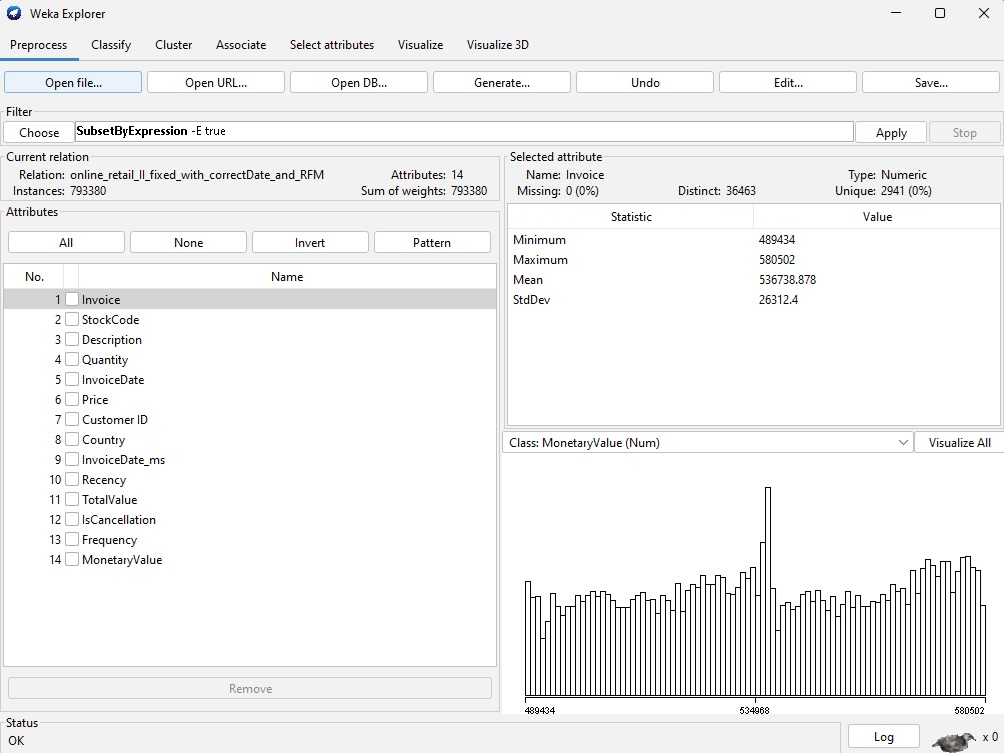
\includegraphics[width=0.7\linewidth]{imagens/figure2.jpg}\label{cap-2-fig2}
    \captionof{figure}[LOF entry]{Janela do Weka após o carregamento inicial do conjunto de dados.}
    \label{fig2}
    \end{centering}
\end{figure}

\vspace{-0.3cm}
Ao terminar o carregamento, podemos notar que o nosso conjunto de dados passou de 1048124 para 793380 instâncias, isto porque anteriormente foram eliminadas as instâncias com o campo \textit{"Customer ID"} vazio e as instâncias que diziam respeito a cancelamentos e devoluções. Podemos reparar que passámos de 8 para 14 atributos, mas muitos destes foram utilizados como atributos temporários pelo \textit{script} Python utilizado anteriormente por forma a calcular os valores de Recência, Frequência e Valor Monetário e como tal deverão ser removidos. Para esse efeito, iremos simplesmente selecionar os atributos a remover no \textit{Weka} e clicar no botão \textit{"Remove"} situado por debaixo da lista de atributos. A figura \ref{fig3} ilustra quais os atributos a remover:
\begin{figure}[H]
    \begin{centering}
    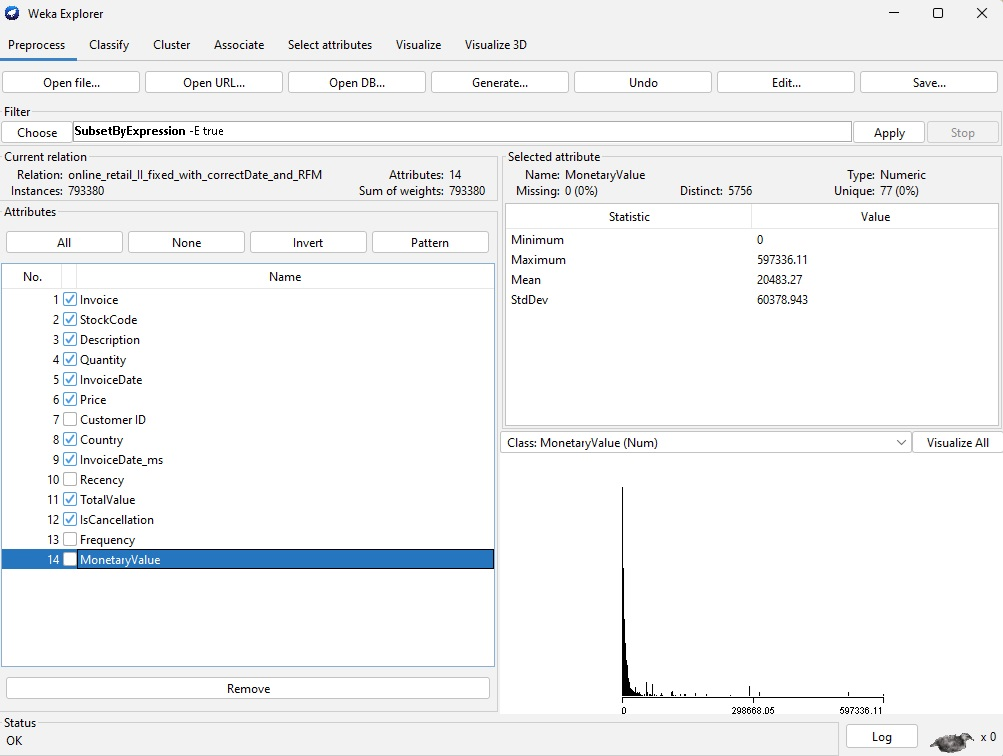
\includegraphics[width=0.7\linewidth]{imagens/figure3.jpg}\label{cap-2-fig3}
    \captionof{figure}[LOF entry]{Indicação dos atributos a remover do conjunto de dados}
    \label{fig3}
    \end{centering}
\end{figure}
Terminada a remoção dos nossos atributos, o próximo passo é a conversão do atributo \textit{"Customer ID"} de numérico para nominal. Para esse efeito, iremos utilizar o filtro \textit{\textbf{NumericToNominal}}, bastando nas opções do mesmo alterar o campo \textit{atributeIndices} e substituir "first-last" por apenas "first". A seguinte figura demonstra essa alteração:

\vspace{-0.2cm}
\begin{figure}[H]
    \begin{centering}
    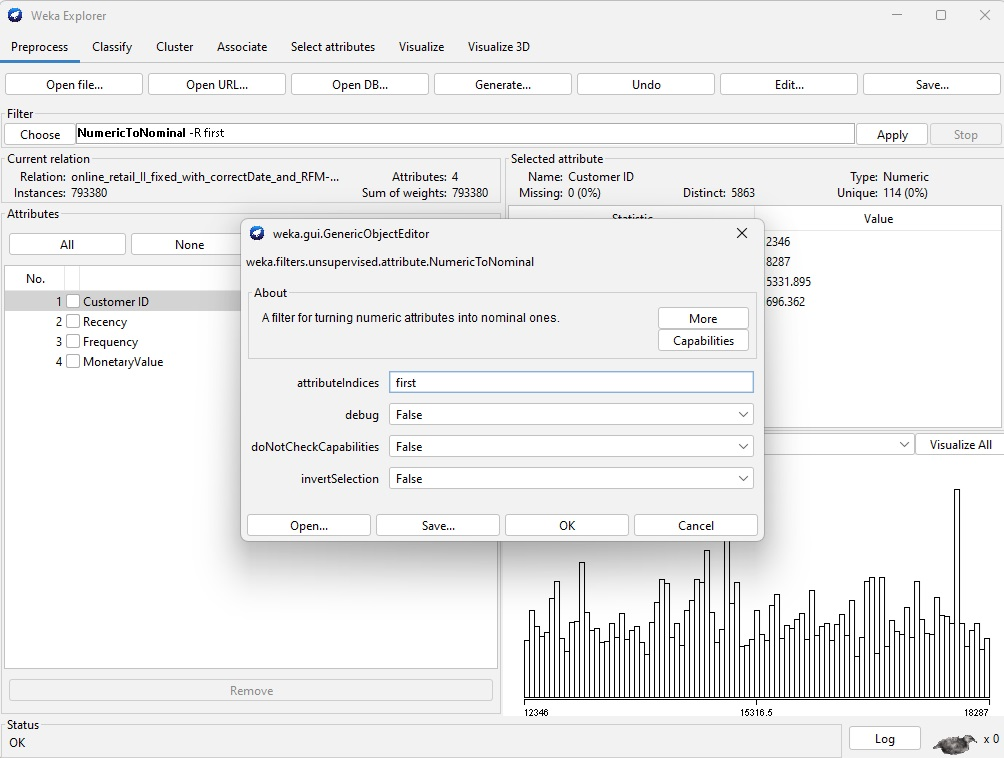
\includegraphics[width=0.63\linewidth]{imagens/figure4.jpg}\label{cap-2-fig4}
    \captionof{figure}[LOF entry]{Opções do filtro \textbf{\textit{NumericToNominal}}.}
    \label{fig4}
    \end{centering}
\end{figure}


\vspace{-0.3cm}
O último passo antes da análise dos dados é a remoção de duplicados. Anteriormente, quando foi feita a remoção de instâncias que diziam respeito a linhas canceladas, foram também calculados os valores de RFM. Estes valores aparecem repetidos por cada instância e por cada cliente, logo removendo os duplicados no \textit{Weka} irá deixar-nos com uma instância por cliente, com os seus valores de RFM. Para podermos realizar esse passo, iremos utilizar o filtro \textbf{\textit{RemoveDuplicates}}. Este filtro não necessita de configurações adicionais, bastando escolher o mesmo e clicar no botão \textit{"Apply"}. A figura seguinte mostra o resultado final da aplicação do filtro:

 \begin{figure}[H]
    \begin{centering}
    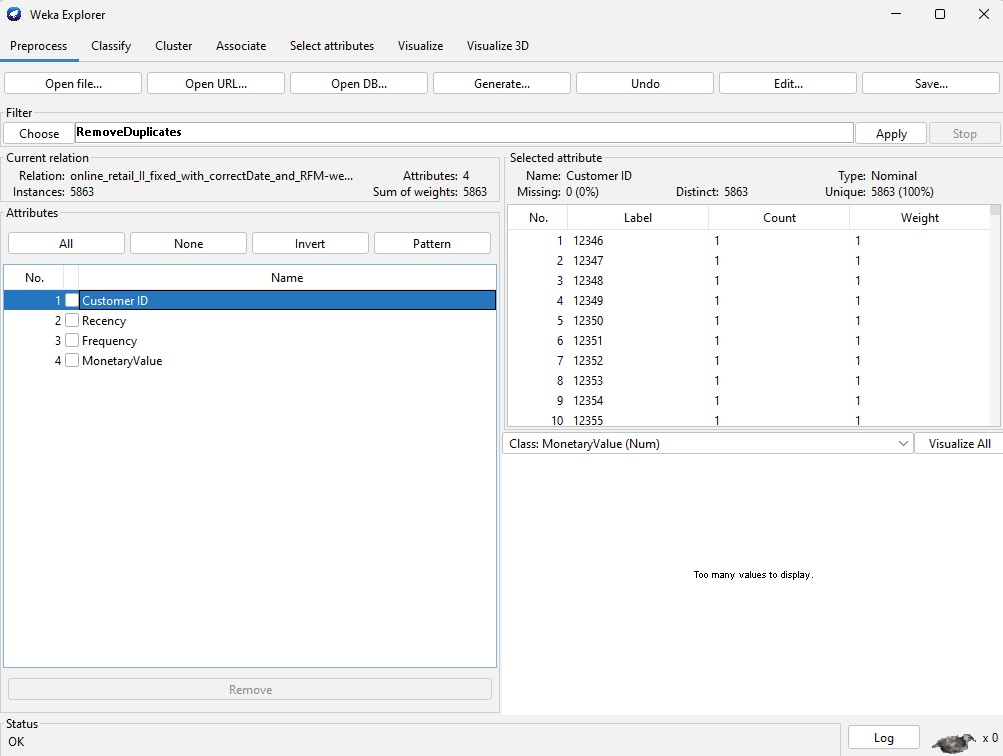
\includegraphics[width=0.63\linewidth]{imagens/figure5.jpg}\label{cap-2-fig5}
    \captionof{figure}[LOF entry]{Resultado final após aplicação do filtro \textit{\textbf{RemoveDuplicates}}.}
    \label{fig5}
    \end{centering}
\end{figure}

Como podemos verificar, a aplicação do filtro \textit{\textbf{RemoveDuplicates}} permitiu-nos reduzir a dimensão do nosso conjunto de dados de 793380 instâncias para apenas 5863. Cada uma das instâncias que permanece diz respeito apenas a um cliente. Caso não se efetuasse a remoção de instâncias duplicadas, ao se aplicar os algoritmos de classificação, estes seriam sobreajustados, pois cada cliente teria multiplas linhas associadas, o que causaria um sobreajuste nas nossas métricas de desempenho.
Agora que os nossos dados estão preparados, iremos passar à segmentação de clientes.

%----------------------------------------------------------------------------------------------------------


%----------------------------------------------------------------------------------------------------------
\section{Segmentação de Clientes}
\subsection{Escolha do número e tipo de \textit{bins}}

Antes de podermos realizar a segmentação de clientes, devemos normalizar os valores de RFM obtidos através da atribuição de pontuações (por exemplo, 1 sendo a pior, 10 sendo a melhor pontuação) para cada métrica. Como os valores de RFM podem variar muito para cada cliente, poderão não ser diretamente comparáveis. Ao atribuirmos pontuações, garantimos que clientes com comportamentos semelhantes sejam colocados no mesmo segmento. Outra vantagem é a mitigação de \textit{outliers}, pois poderão existir clientes com valores muito altos de Recência, Frequência e/ou valor Monetário que irão causar distorção nos nossos dados.
Para realizarmos a atribuição de pontuações, devemos discretizar os nossos dados em \textit{bins}. Para isso, podemos utilizar o \textit{software} \textit{\textbf{Weka}}, através do filtro \textit{\textbf{Discretize}}. No entanto, devemos olhar primeiro para os valores a discretizar, para verificarmos as distribuições dos seus valores e decidir se deveremos aplicar \textit{equal-frequency binning} ou \textit{equal-width binning}. Abaixo podemos encontrar gráficos que ilustram a distribuião dos nossos dados:

 \begin{figure}[H]
    \begin{centering}
    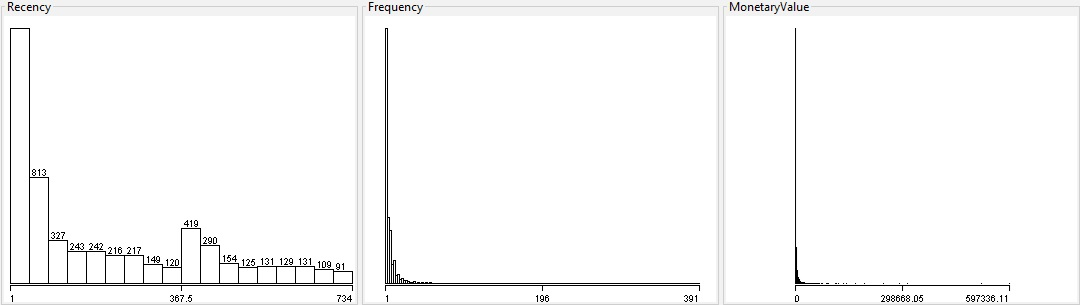
\includegraphics[width=1\linewidth]{imagens/figure6.jpg}\label{cap-3-fig6}
    \captionof{figure}[LOF entry]{Distribuições dos clientes por Recência, Frequência e valor Monetário.}
    \label{fig6}
    \end{centering}
\end{figure}

Como podemos verificar, existe uma grande discrepância nos valores de cada uma das métricas:

\begin{enumerate}
    \item \textbf{Recência}: Existe uma grande diferença entre os valores, com grande parte dos clientes tendo um valor de recência baixo, ou seja, esses clientes realizaram compras recentemente.
    \item \textbf{Frequência}: Existe uma grande diferença entre os valores, com grande parte dos clientes tendo um valor de Frequência baixo, ou seja, esses clientes realizaram compras pouco frequentemente.
    \item \textbf{Valor Monetário}: Existe uma grande diferença entre os valores, grande parte dos clientes  realizou compras cujo valor total é baixo, existem clientes com valores monetários muito baixos, provavelmente atacadistas (clientes que compram em grandes quantidades, possivelmente para revenda).
\end{enumerate}

Para podermos colmatar este problema, é recomendada a utilização de \textbf{\textit{equal-frequency binning}} \cite{RFMSDM2004}. Como os nossos dados não estão uniformemente distribuidos, a utilização desse tipo de separação irá permitir que cada \textit{bin} tenha aproximadamente o mesmo número de clientes,o que irá permitir balancear os segmentos de utilizador e permitir uma comparabilidade melhorada em todas as métricas.
O próximo passo é a decisão do número de \textit{bins}. Em teoria, quanto maior for o número de bins, melhor será a granularidade da nossa análise em segmentar os clientes, mas esse aumento da granularidade irá diminuir a nossa capacidade de interpretar os resultados finais e segmentar os clientes de acordo com a sua pontuação. Por exemplo, com a divisão em \textit{bins} de tamanho 10, se fossemos a mostrar os segmentos de clientes num gráfico 2D (Recência \textit{vs.} Frequência), teriamos uma grelha de tamanho 100 (10x10). O problema torna-se mais complexo se adicionarmos uma terceira dimensão (valor monetário), teriamos 1000 (10x10x10) zonas diferentes no gráfico de segmentos de clientes. 
Para efeitos da análise realizada ao conjunto de dados neste documento, iremos então escolher um número de \textit{bins} mais modesto, com a discretização a ser efetuada com 5 \textit{bins}. Com esta separação, o gráfico 2D da nossa análise, quando compararmos Recência \textit{vs.} Frequência, terá 25 zonas (5x5), o gráfico 3d será composto por 125 zonas (5x5x5).


\subsection{Discretização e atribuição de pontuações RFM}

Antes de aplicarmos a discretização dos nossos atributos, devemos criar uma cópia dos mesmos por forma a não se perder os valores originais de RFM. Para isso, devemos utilizar o filtro \textit{\textbf{AddExpression}} da seguinte forma, para cada um dos atributos:

 \begin{figure}[H]
    \begin{centering}
    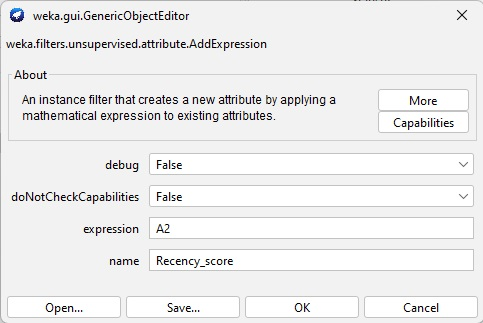
\includegraphics[width=0.5\linewidth]{imagens/figure12.jpg}\label{cap-3-fig12}
    \captionof{figure}[LOF entry]{Aplicação do filtro \textit{\textbf{AddExpression}} para o atributo \textit{Recency}.}
    \label{fig12}
    \end{centering}
\end{figure}

 \begin{figure}[H]
    \begin{centering}
    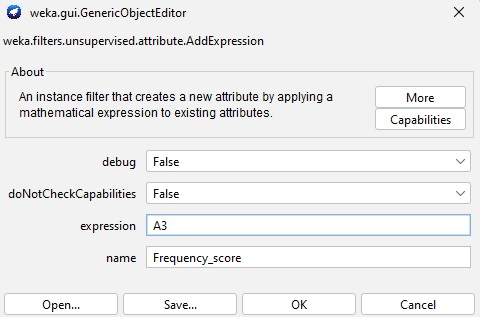
\includegraphics[width=0.5\linewidth]{imagens/figure13.jpg}\label{cap-3-fig13}
    \captionof{figure}[LOF entry]{Aplicação do filtro \textit{\textbf{AddExpression}} para o atributo \textit{Frequency}.}
    \label{fig13}
    \end{centering}
\end{figure}

 \begin{figure}[H]
    \begin{centering}
    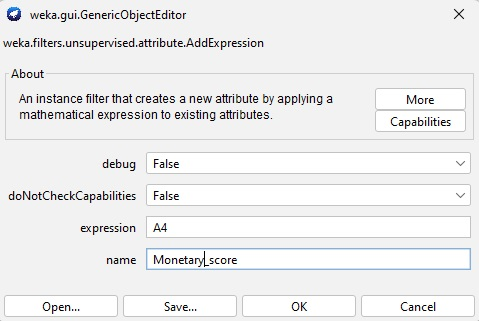
\includegraphics[width=0.5\linewidth]{imagens/figure14.jpg}\label{cap-3-fig14}
    \captionof{figure}[LOF entry]{Aplicação do filtro \textit{\textbf{AddExpression}} para o atributo \textit{Monetary Value}.}
    \label{fig14}
    \end{centering}
\end{figure}

Após a criação das cópias dos nossos atributos RFM, iremos aplicar a discretização aos mesmos. Anteriormente, ficou decidida a utilização de \textit{\textbf{equal-frequency binning}} com 5 \textit{bins}. Para podermos realizar essa operação, iremos utilizar o \textit{Weka}, mais específicamete o seu fitro \textit{\textbf{Discretize}}. A figura \ref{fig7} demonstra a aplicação do filtro, bem como os parâmetros a ser definidos:

 \begin{figure}[H]
    \begin{centering}
    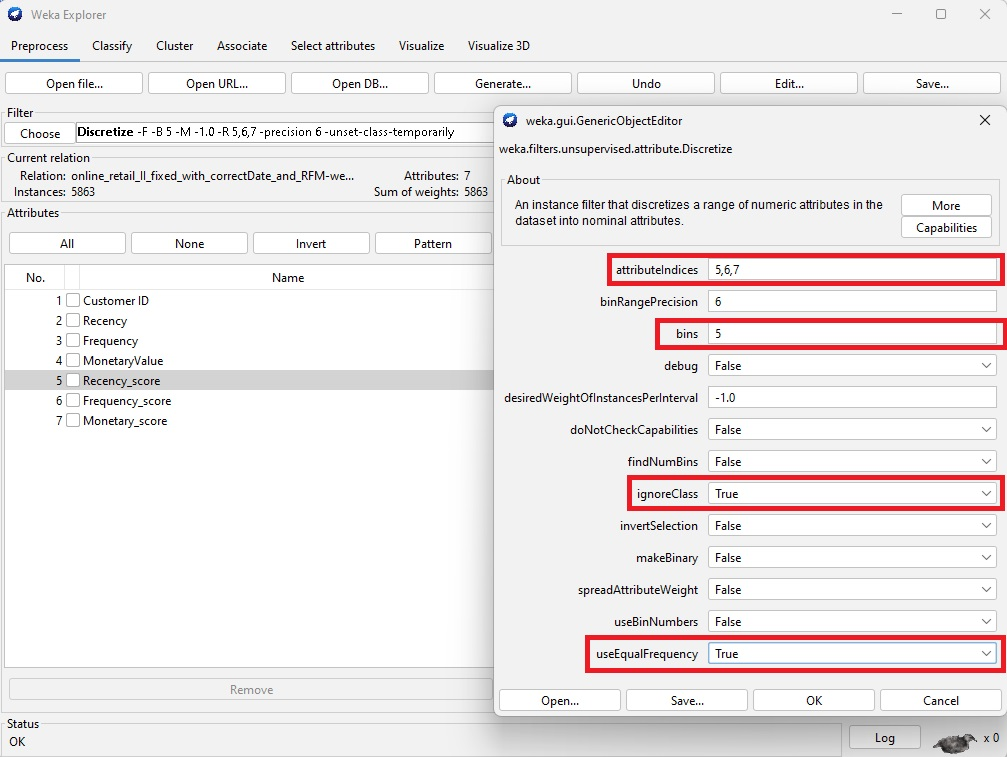
\includegraphics[width=1\linewidth]{imagens/figure7.jpg}\label{cap-4-fig7}
    \captionof{figure}[LOF entry]{Distribuições dos clientes por Recência, Frequência e valor Monetário.}
    \label{fig7}
    \end{centering}
\end{figure}

\begin{enumerate}
    \item \textbf{\textit{atributesIndices}}: Nesta opção, indicamos quais os índices dos atributos aos quais queremos aplicar a discretização. Devemos colocar "5,6,7" (sem as aspas).
    \item \textbf{\textit{bins}}: Nesta opção, é feita a definição do número de \textit{bins}. Para efeitos deste artigo, iremos utilizar 5 \textit{bins}.
    \item \textbf{\textit{ignoreClass}}: Nesta opção, indicamos que queremos ignorar o atributo classe. Escolhemos \textit{"True"}.
    \item \textbf{\textit{useEqualFrequency}}: Nesta opção, indicamos que queremos realizar o \textit{binning} com \textit{equal-frequency binning}.
\end{enumerate}

Depois de aplicarmos a discretização, os valores de Recência, Frequência e Valor Monetário serão agrupados em 5 \textit{bins} de acordo com a sua frequência. A figura \ref{fig8} mostra o resultado final da discretização:

\begin{figure}[H]
    \begin{centering}
    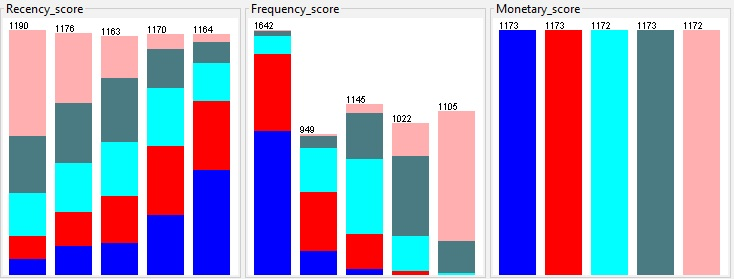
\includegraphics[width=0.9\linewidth]{imagens/figure8.jpg}\label{cap-4-fig8}
    \captionof{figure}[LOF entry]{Distribuições dos clientes por Recência, Frequência e valor Monetário, por 5 \textit{bins}.}
    \label{fig8}
    \end{centering}
\end{figure}

Como podemos verificar, a utilização de \textit{\textbf{equal-frequency binning}} permitiu-nos balancear os dados, criando células com o número aproximado de clientes. Apenas no caso da Frequência é que houve um menor balanceamento, mas isso poderá ser explicado pela grande diferença entre os hábitos de compras dos clientes, com grande prevalência de clientes com poucas compras realizadas.

O próximo passo é o renomear dos \textit{bins} obtidos para valores numéricos de 1 a 5, em que valores mais altos indicam pontuação mais elevada:

\begin{enumerate}
	\item[\textbullet] \textbf{Recência}: Quanto menor a recência, melhor a pontuação.
	\item[\textbullet] \textbf{Frequência}: Quanto maior a frequência, melhor a pontuação.
	\item[\textbullet] \textbf{Valor Monetário}: Quanto maior o valor monetário, melhor a pontuação.
\end{enumerate}

Para realizarmos a operação de renomear os diferentes \textit{bins} iremos utilizar o filtro \textit{\textbf{RenameNominalValues}}. Este filtro permite indicar os valores a substituir e o seu substituto, podendo realizar multiplas substituições de uma vez só. Para cada um dos atributos RFM, iremos realizar as seguintes substituições:

\begin{enumerate}
	\item \textbf{Recência}:
		\item[\textbullet] \textbf{(-inf-19.5]}: 5
		\item[\textbullet] \textbf{(19.5-59.5]}: 4
		\item[\textbullet] \textbf{(59.5-193.5]}: 3
		\item[\textbullet] \textbf{(193.5-406.5]}: 2
		\item[\textbullet] \textbf{(406.5-inf)}: 1
	\item \textbf{Frequência}:
		\item[\textbullet] \textbf{(-inf-1.5]}: 1
		\item[\textbullet] \textbf{(1.5-2.5]}: 2
		\item[\textbullet] \textbf{(2.5-4.5]}: 3
		\item[\textbullet] \textbf{(4.5-8.5]}: 4
		\item[\textbullet] \textbf{(8.5-inf)}: 5
	\item \textbf{Valor Monetário}:
		\item[\textbullet] \textbf{(-inf-285.67]}: 1
		\item[\textbullet] \textbf{(285.67-612.69]}: 2
		\item[\textbullet] \textbf{(612.69-1231.44]}: 3
		\item[\textbullet] \textbf{(1231.44-2932.06]}: 4
		\item[\textbullet] \textbf{(2932.06-inf)}: 5
\end{enumerate}


Abaixo podemos encontrar a aplicação do filtro para todos os atributos RFM:

\begin{figure}[H]
    \begin{centering}
    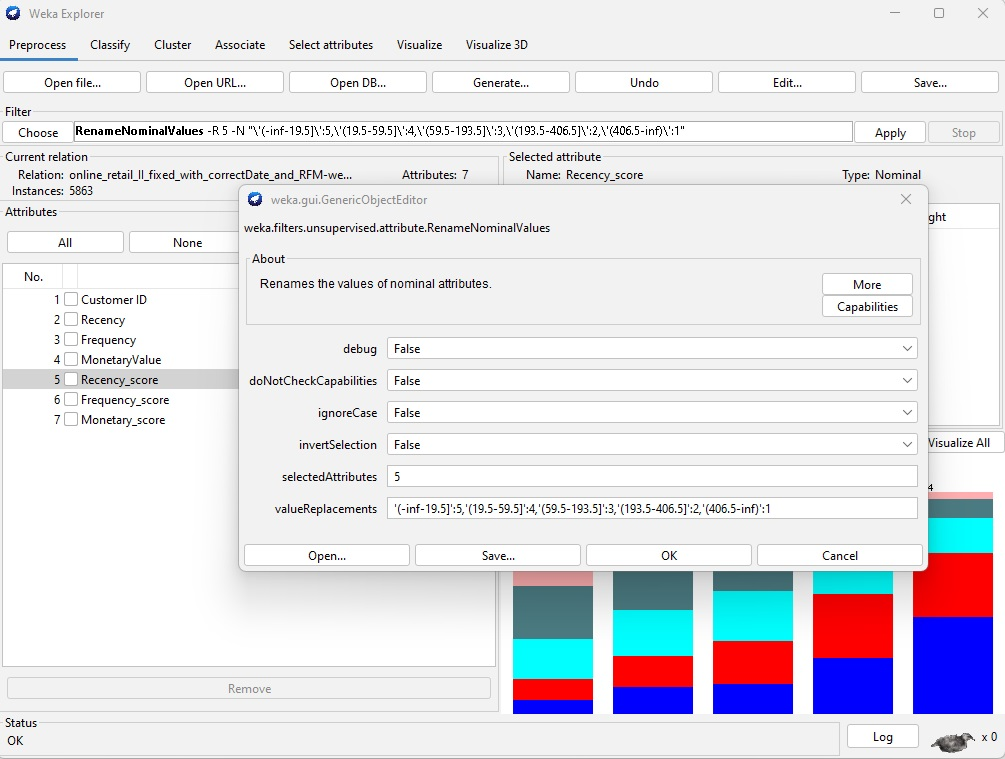
\includegraphics[width=0.85\linewidth]{imagens/figure9.jpg}\label{cap-3-fig9}
    \captionof{figure}[LOF entry]{Alteração do nome dos intervalos de Recência para refletir a pontuação.}
    \label{fig9}
    \end{centering}
\end{figure}

\begin{figure}[H]
    \begin{centering}
    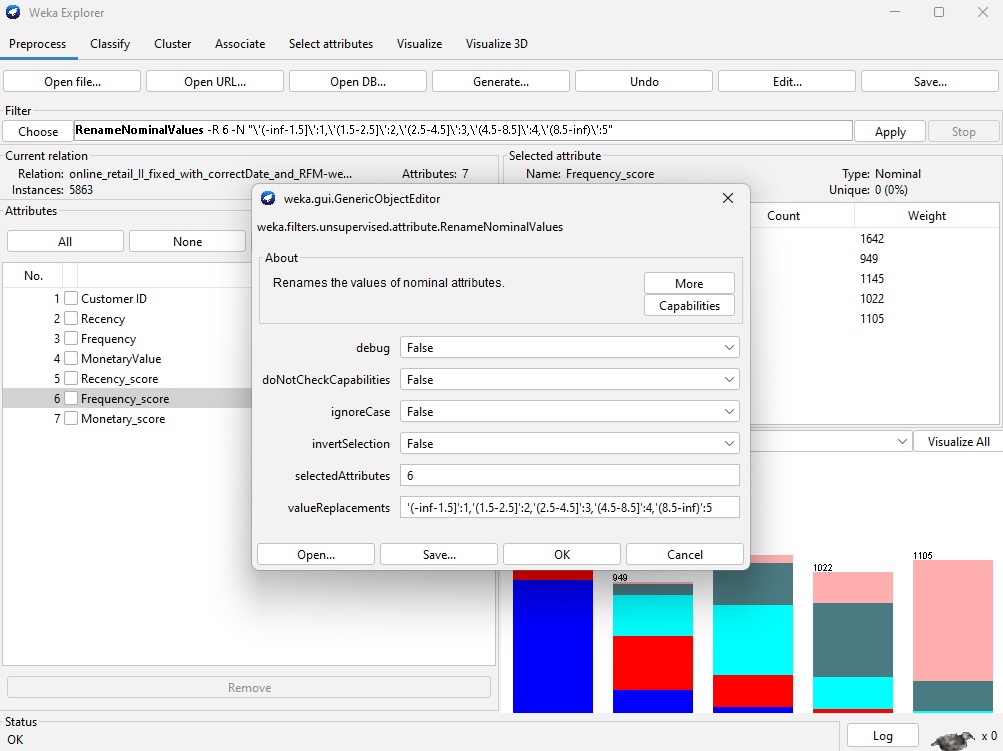
\includegraphics[width=0.85\linewidth]{imagens/figure10.jpg}\label{cap-3-fig10}
    \captionof{figure}[LOF entry]{Alteração do nome dos intervalos de Frequência para refletir a pontuação.}
    \label{fig10}
    \end{centering}
\end{figure}

\begin{figure}[H]
    \begin{centering}
    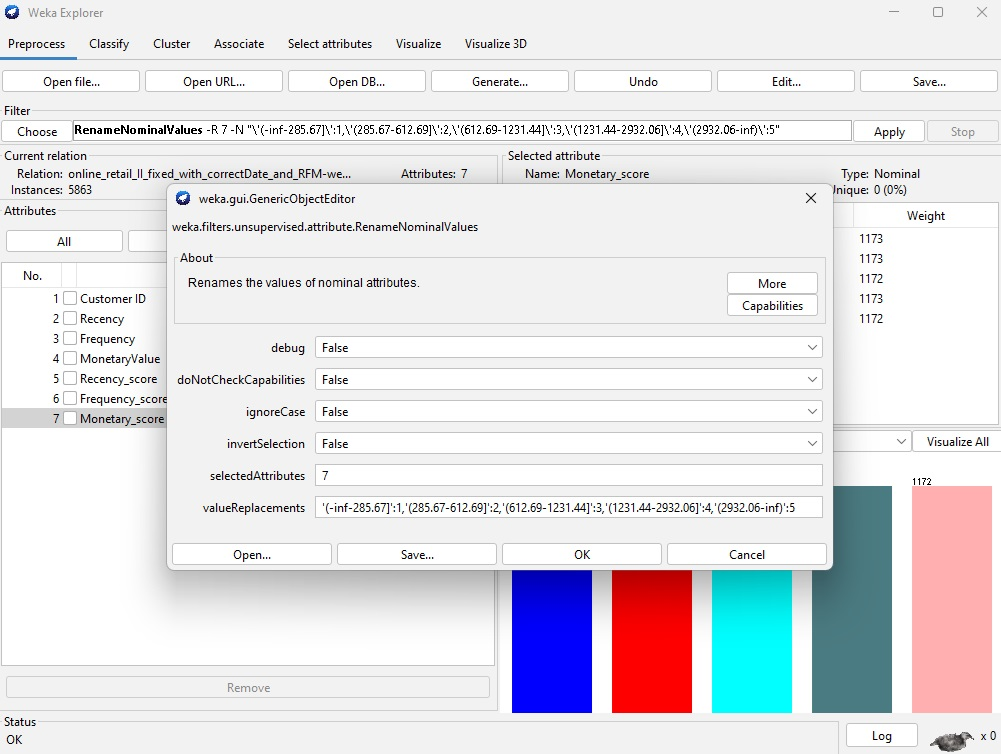
\includegraphics[width=0.85\linewidth]{imagens/figure11.jpg}\label{cap-3-fig11}
    \captionof{figure}[LOF entry]{Alteração do nome dos intervalos do valor Monetário para refletir a pontuação.}
    \label{fig11}
    \end{centering}
\end{figure}

O próximo passo é a segmentação dos clientes de acordo com os valores de pontuação RFM. Para isso, devemos converter primeiro os atributos de pontuação de nominal para numéricos. Uma forma simples de o fazer sem recorrer a nenhum filtro no \textit{Weka} é guardar o trabalho realizado até aqui como um ficheiro .arff, abrir o ficheiro num editor de texto e alterar o tipo de dados no cabeçalho para os atributos \textit{\textbf{Recency_score}}, \textit{\textbf{Frequency_score}} e \textit{\textbf{Monetary_score}} de \textit{\textbf{nominal}} (removendo a lista de atributos nominais) para \textit{\textbf{numeric}}.

\begin{figure}[H]
    \begin{centering}
    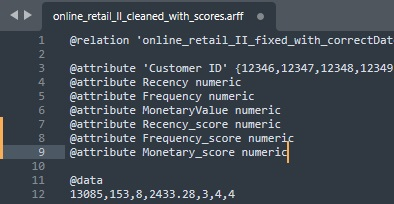
\includegraphics[width=0.85\linewidth]{imagens/figure15.jpg}\label{cap-3-fig15}
    \captionof{figure}[LOF entry]{Alteração do tipo de dados das pontuações RFM de nominal para numérico com o editor \textit{\textbf{Sublime Text}}.}
    \label{fig15}
    \end{centering}
\end{figure}

\newpage
Quando voltarmos a abrir o \textit{Weka}, os nossos atributos já serão interpretados como atributos numéricos. De seguida, iremos proceder à segmentação dos clientes com base nos valores de pontuação RFM, utilizando para esse efeito o \textit{\textbf{K-means Clustering}}. No entanto, será necessário escolher o número de segmentos de cliente com base nas pontuações. Para esse efeito, iremos utilizar o chamado \textit{\textbf{Elbow Method}}\cite{RCCAFRM}.
O \textit{\textbf{Elbow Method}} ajuda-nos a identificar o \textit{tradeoff} ótimo entre a complexidade do modelo e a variância explicada (a similaridade intra-\textit{cluster}). Além disso, a utilização de demasiados \textit{clusters} pode causar o sobreajustamento dos nossos dados (o chamado \textit{overfit}), em que são criados \textit{clusters} pequenos que não têm capacidade de generalização.
Testando multiplos valores de K na aba \textit{\textbf{Cluster}} no \textit{Weka}, obtemos o seguinte resultado:

\begin{table}[htb]
\centering
\begin{tabular}{l|l|l|l}
Número de Clusters & Within Cluster Sum of Squared Errors  & Diferença &   \\
\hline
2                  & 989.8093476                                    &         &   \\
3                  & 755.0489622                                    & -23.7177\%  &   \\
4                  & 540.0345318                                    & -28.4769\% &   \\
5                  & 457.3705245                                    & -15.3072\%  &   \\
6                  & 407.868599                                     & -10.8232\%  &   \\
7                  & 369.9222038                                    & -9.30358\%  &   \\
8                  & 348.0911701                                    & -5.90152\%  &   \\
9                  & 321.9408009                                    & -7.51251\%  &   \\
10                 & 285.7621183                                    & -11.2377\%  &  
\end{tabular}
\end{table}

\begin{figure}[H]
    \begin{centering}
    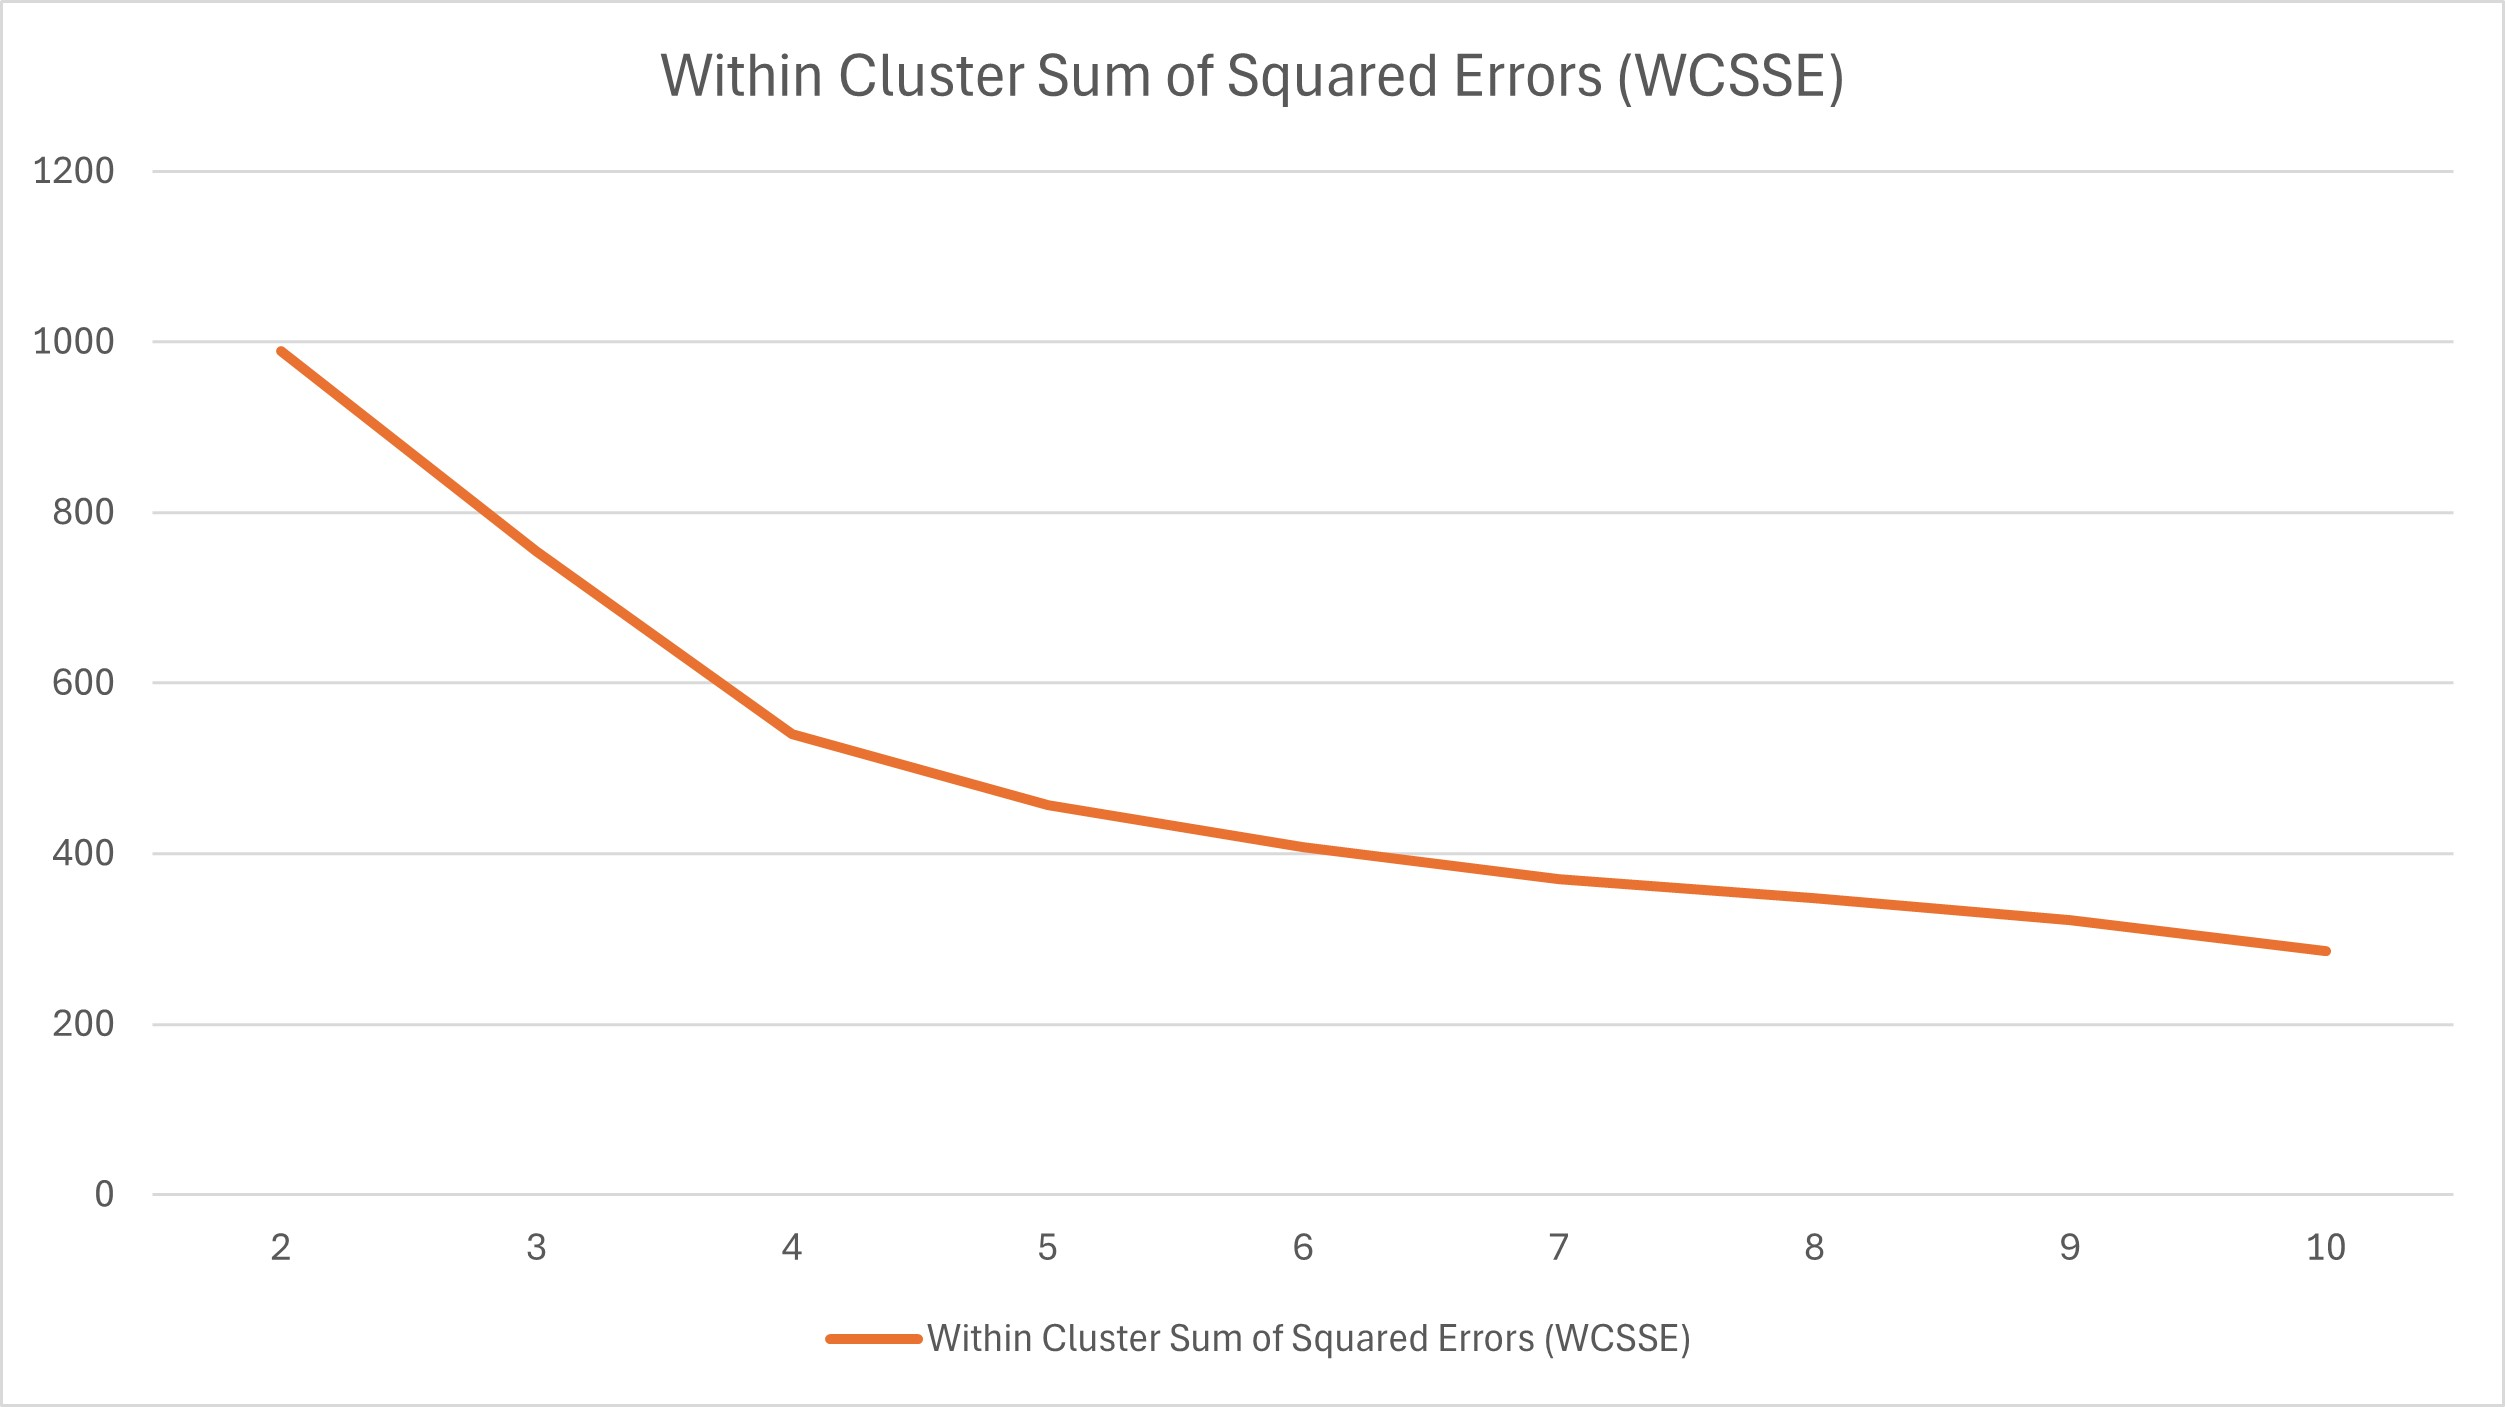
\includegraphics[width=1\linewidth]{imagens/figure16.jpg}\label{cap-3-fig16}
    \captionof{figure}[LOF entry]{Curva que ilustra a redução cada vez mais expressiva nos valores de erro.}
    \label{fig16}
    \end{centering}
\end{figure}


\newpage
Com base nos resultados anteriores, iremos escolher o valor de 5 para o número de \textit{clusters}, dado que valores superiores de K oferecem um ganho cada vez mais diminuto.
A segmentação de clientes pode ser definida então como uma questão de troca (\textit{tradeoff}) ou balanceamento entre a granularidade da análise e a sua complexidade. Com a utillização de 5 \textit{clusters}, a nossa segmentação de clientes irá ter em conta apenas 5 grupos distintos de clientes:

\begin{enumerate}
    \item \textbf{Clientes VIP}: Estes são os melhores clientes, que compram frequentemente, gastam muito e realizaram compras recentemente.
		\item[\textbullet] \textbf{Recência}: Muito recente.
		\item[\textbullet] \textbf{Frequência}: Muito frequente.
		\item[\textbullet] \textbf{Valor Monetário}: Muito alto.
    \item \textbf{Clientes Fiéis}: Estes clientes compram regilarmente, mas gastam de forma moderada.
		\item[\textbullet] \textbf{Recência}: Recente.
		\item[\textbullet] \textbf{Frequência}: Muito frequente.
		\item[\textbullet] \textbf{Valor Monetário}: Moderado.
    \item \textbf{Grandes Gastadores Ocasionais}: Estes clientes gastam muito quando compram, mas fazem-no raramente.
		\item[\textbullet] \textbf{Recência}: Moderado.
		\item[\textbullet] \textbf{Frequência}: Pouco Frequente.
		\item[\textbullet] \textbf{Valor Monetário}: Muito alto.
    \item \textbf{Clientes em Risco}: Estes clientes compraram no passado, mas não retornaram recentemente.
		\item[\textbullet] \textbf{Recência}: Antigo.
		\item[\textbullet] \textbf{Frequência}: Pouco Frequente.
		\item[\textbullet] \textbf{Valor Monetário}: Baixo a moderado.
    \item \textbf{Clientes Perdidos}: Não compram a muito tempo, gastaram pouco e compraram raramente.
		\item[\textbullet] \textbf{Recência}: Muito Antigo.
		\item[\textbullet] \textbf{Frequência}: Infrequente.
		\item[\textbullet] \textbf{Valor Monetário}: Muito Baixo.
\end{enumerate}

\newpage

Agora que escolhemos o número de clusters, iremos voltar ao \textit{Weka} e iremos seleccionar o filtro \textit{\textbf{AddCluster}}. Na opção \textit{\textbf{ignoreAttributeIndices}}, escolhemos ignorar todos os atributos que não sejam as pontuações RFM, conforme a imagem abaixo:

\begin{figure}[H]
    \begin{centering}
    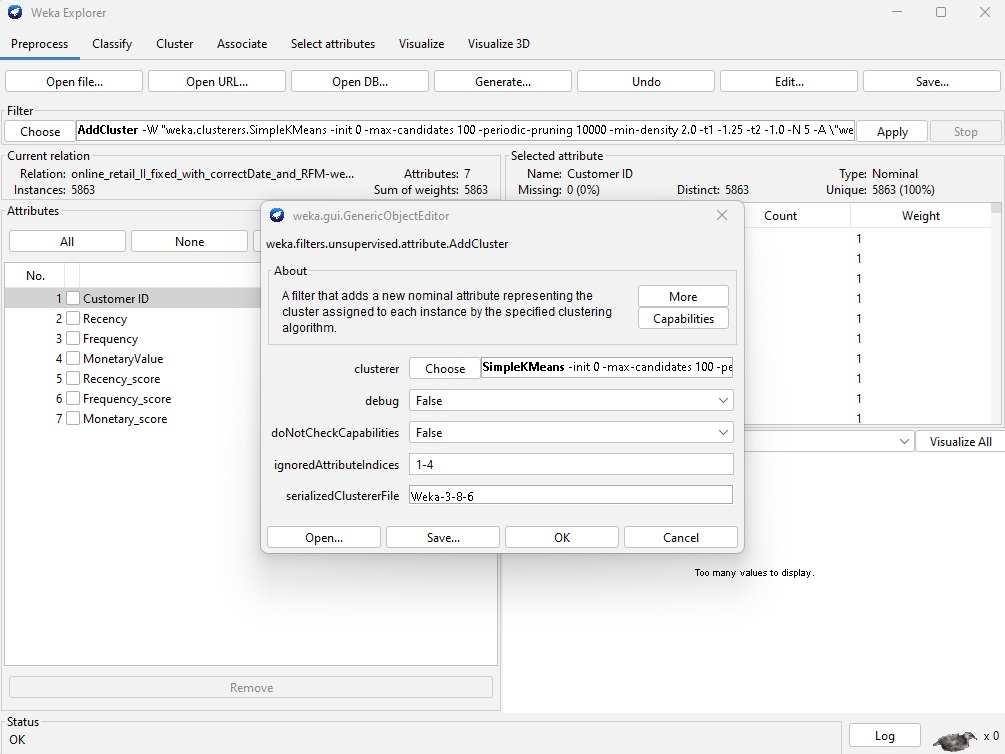
\includegraphics[width=0.6\linewidth]{imagens/figure17.jpg}\label{cap-3-fig17}
    \captionof{figure}[LOF entry]{Opções do filtro \textit{\textbf{AddCluster}}.}
    \label{fig17}
    \end{centering}
\end{figure}

De seguida, abrimos as opções do algoritmo de \textit{Clustering} e escolhemos na opção \textit{numClusters}, colocando o valor 5:

\begin{figure}[H]
    \begin{centering}
    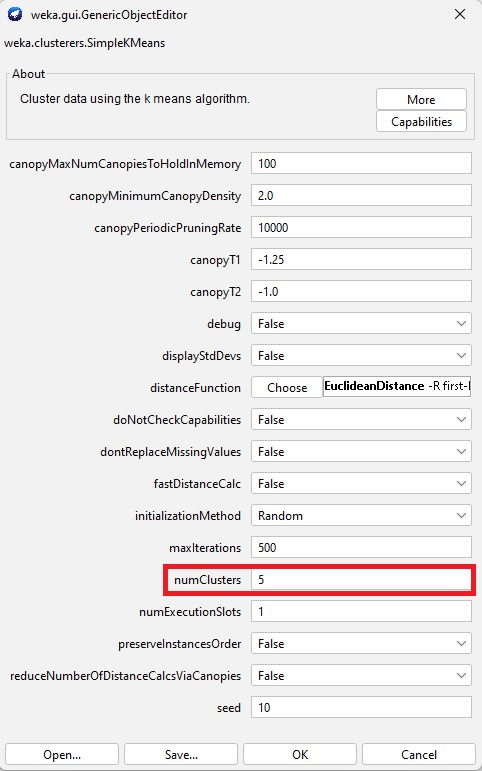
\includegraphics[width=0.4\linewidth]{imagens/figure18.jpg}\label{cap-3-fig18}
    \captionof{figure}[LOF entry]{Opções do filtro \textit{\textbf{AddCluster}}.}
    \label{fig18}
    \end{centering}
\end{figure}

Depois de aplicarmos o \textit{clustering} ao nosso conjunto de dados, obtemos a seguinte distribuição de instâncias por cada um dos \textit{clusters} (mais tarde iremos renomear cada um para que os nomes coincidam com os grupos definidos acima, mas primeiro precisamos de identificar cada um dos grupos):


\begin{figure}[H]
    \begin{centering}
    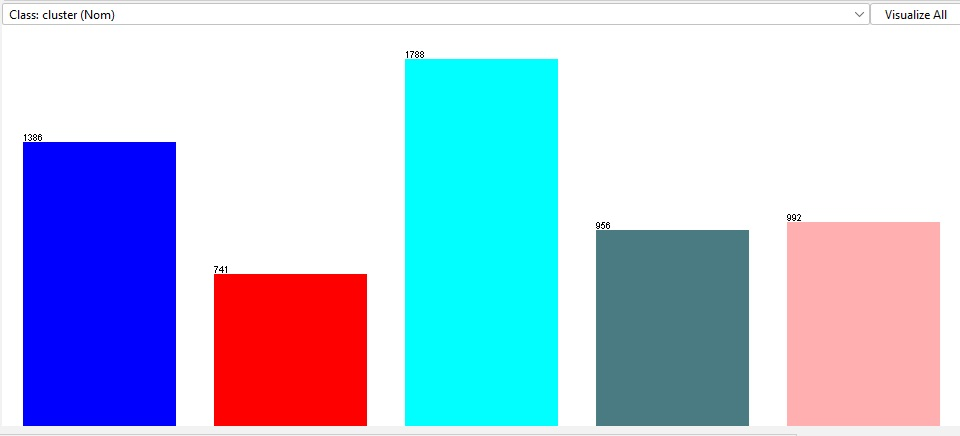
\includegraphics[width=1\linewidth]{imagens/figure19.jpg}\label{cap-3-fig19}
    \captionof{figure}[LOF entry]{Distribuição de instâncias por cada \textit{cluster}.}
    \label{fig19}
    \end{centering}
\end{figure}

\subsection{Cálculo do Risco de Abandono}

Outra métrica muito importante na análise RFM é o chamado risco de abandono de clientes (em inglês, \textit{\textbf{customer churn}}). Esta métrica indica a probabilidade que cada cliente tem, com base no seu histórico anterior, de vir a abandonar o negócio do qual o conjunto de dados diz respeito num futuro próximo.
Com base na informação do \textit{\textbf{churn}}, as empresas poderão definir estratégias para reter os clientes em risco.
Para calcular um valor normalizado na escala de [0...1] do risco de \textit{churn} para cada cliente, podemos utilizar a seguinte formula:

\[ \textit{ChurnRisk} = w_R*(1-\frac{RecencyScore}{Max(RecencyScore)}) + w_F*(1-\frac{FrequencyScore}{Max(FrequencyScore)}) + w_M*(1-\frac{MonetaryScore}{Max(MonetaryScore)})\]


Em que:

\begin{enumerate}
	\item[\textbullet] \textit{\textbf{ChurnRisk}}: Corresponde ao valor de risco de abandono normalizado, entre [0...1].
	\item[\textbullet] \textit{\textbf{wR}}: Corresponde a um valor de peso a atribuir à pontuação normalizada referente à recência, na escala de [0...1].
	\item[\textbullet] \textit{\textbf{wF}}: Corresponde a um valor de peso a atribuir à pontuação normalizada referente à frequência, na escala de [0...1].
	\item[\textbullet] \textit{\textbf{wM}}: Corresponde a um valor de peso a atribuir à pontuação normalizada referente ao valor monetário, na escala de [0...1].
	\item[\textbullet] \textit{\textbf{RecencyScore}}: Corresponde ao valor de pontuação atribuido à recência de determinado cliente, na escala de [1...5].
	\item[\textbullet] \textit{\textbf{FrequencyScore}}: Corresponde ao valor de pontuação atribuido à frequência de determinado cliente, na escala de [1...5].
	\item[\textbullet] \textit{\textbf{MonetaryScore}}: Corresponde ao valor de pontuação atribuido ao valor monetário de determinado cliente, na escala de [1...5].
	\item[\textbullet] \textit{\textbf{Max(.......)}}: Corresponde ao valor máximo de pontuação relativo a cada uma das componentes RFM. No caso deste conjunto de dados, o valor é sempre 5.
\end{enumerate}

\textit{\textbf{\underline{Nota:}}}: A soma dos pesos wR, wF e wM deve de ser igual a 1, caso contrário arriscamos a subajustar ou sobreajustar o nosso modelo. A escolha de qual valor de pesos a aplicar irá depender da estratégia empresarial de cada organização, caso queiram dar mais enfâse à recência, frequência ou valor monetário das compras dos seus clientes. Para continuar o teste ao conjunto de dados deste artigo, iremos definir wR = 0.5, wF = 0.3 e wM = 0.2.
Para aplicarmos a fórmula acima a cada instância dos nossos dados, iremos utilizar novamente o filtro \textit{\textbf{AddExpression}}, criando um novo atributo chamado \textit{\textbf{ChurnRisk}}:

\begin{figure}[H]
    \begin{centering}
    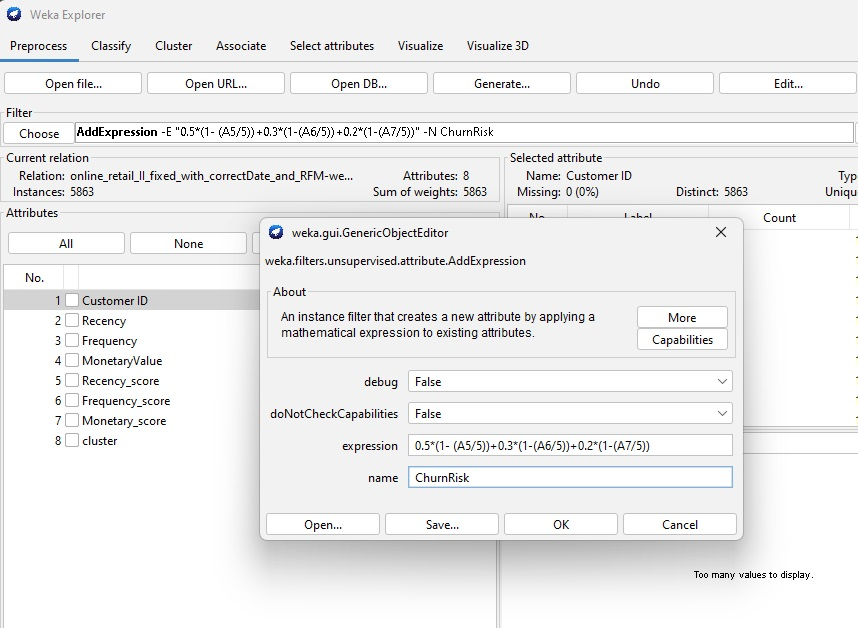
\includegraphics[width=1\linewidth]{imagens/figure20.jpg}\label{cap-3-fig20}
    \captionof{figure}[LOF entry]{Criação do novo atributo \textit{\textbf{ChurnRisk}}.}
    \label{fig20}
    \end{centering}
\end{figure}

Após aplicarmos o filtro, cada uma das instâncias terá um novo atributo numérico na escala de [0...1] que indica a probabilidade do cliente abandonar o negócio. O próximo passo será definir intervalos e um novo atributo nominal que indique qual o nível de risco (Baixo Risco, Alto Risco, ...). Para isso, voltamos a utilizar o filtro \textit{\textbf{AddExpression}} com a seguinte expressão:

\begin{figure}[H]
    \begin{centering}
    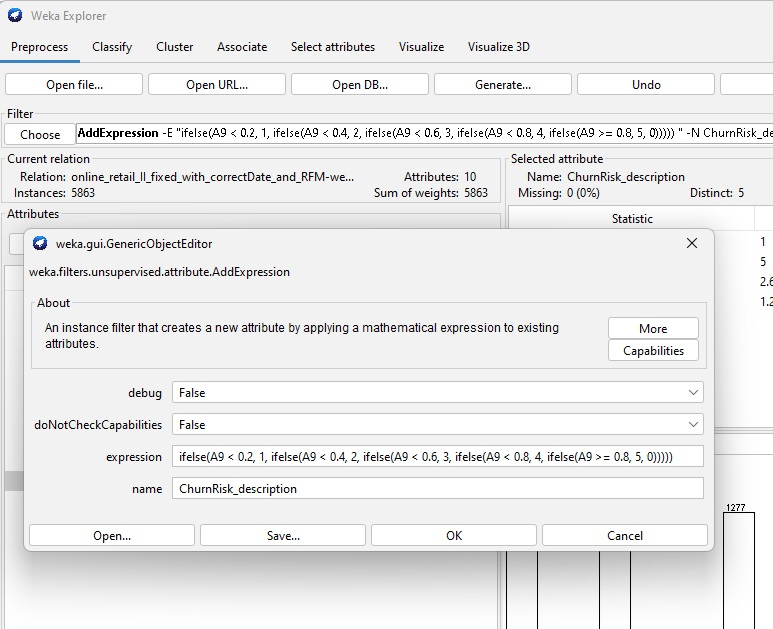
\includegraphics[width=1\linewidth]{imagens/figure21.jpg}\label{cap-3-fig21}
    \captionof{figure}[LOF entry]{Definição de intervalos de risco por cliente.}
    \label{fig21}
    \end{centering}
\end{figure}

De momento, este filtro criou um novo atributo numérico com valores entre 1 e 5, que indicam o nível de risco. No entanto, para ser mais legível, iremos converter o atributo de numérico para nominal e substituir os números por descrições mais facilmente interpretáveis. Para tal, iremos aplicar o filtro \textit{\textbf{NumericToNominal}}, escolhendo o atributo \textit{last}:

\begin{figure}[H]
    \begin{centering}
    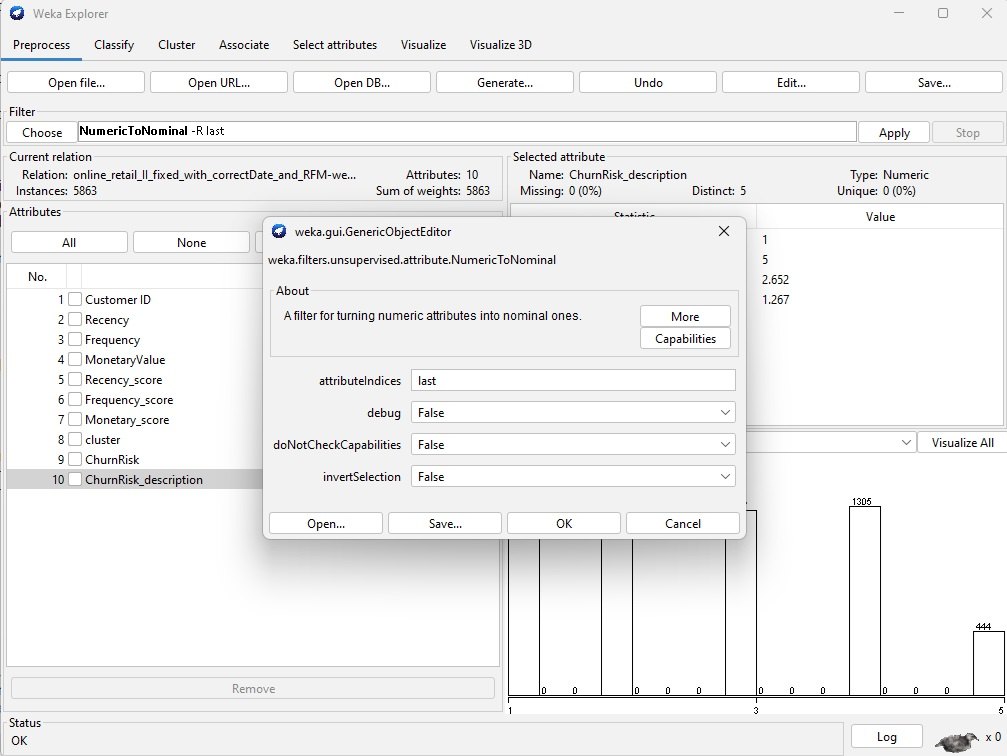
\includegraphics[width=1\linewidth]{imagens/figure22.jpg}\label{cap-3-fig22}
    \captionof{figure}[LOF entry]{Conversão do atributo \textit{\textbf{ChurnRisk_description}} de numérico para nominal.}
    \label{fig22}
    \end{centering}
\end{figure}

O último passo é a renomeação dos diferentes valores nominais de [1...5] numa descrição mais interpretável. Para isso, será necessário voltar a aplicar o filtro \textit{\textbf{RenameNominalValues}}, definindo as seguintes descrições por cada nível:

\begin{enumerate}
	\item[\textbullet] \textbf{1}: Muito Baixo Risco.
	\item[\textbullet] \textbf{2}: Baixo Risco.
	\item[\textbullet] \textbf{3}: Médio Risco.
	\item[\textbullet] \textbf{4}: Alto Risco.
	\item[\textbullet] \textbf{5}: Muito Alto Risco.
\end{enumerate}

\newpage
A figura seguinte ilustra a aplicação do nosso filtro de acordo com as regras acima:

\begin{figure}[H]
    \begin{centering}
    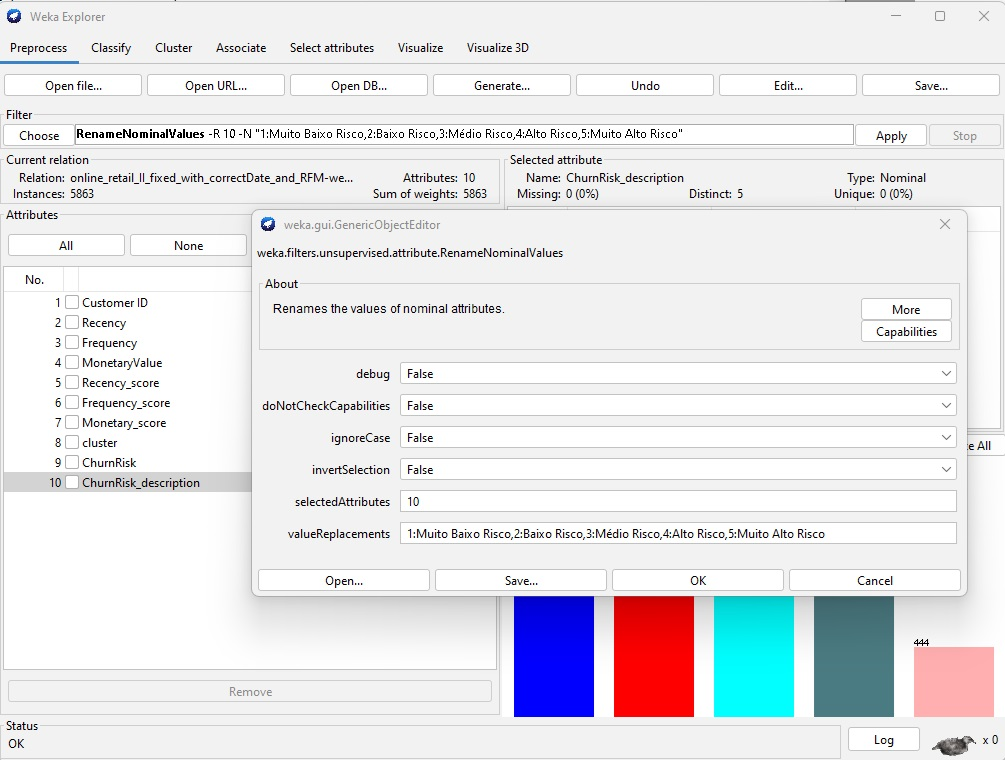
\includegraphics[width=1\linewidth]{imagens/figure23.jpg}\label{cap-3-fig23}
    \captionof{figure}[LOF entry]{Renomeação dos atributos nominais.}
    \label{fig23}
    \end{centering}
\end{figure}

\section{}


%----------------------------------------------------------------------------------------------------------
\bibliographystyle{plain}
\bibliography{artigo}

\end{document}